\documentclass[10pt]{beamer}

\usetheme{Boadilla}
\usecolortheme{default}
\setbeamertemplate{navigation symbols}{}

\usepackage[T1]{fontenc}
\usepackage[utf8]{inputenc}
\usepackage{booktabs}
\usepackage{graphicx}
\usepackage{amsmath}

\title[LTD Reproduction]{Reproducing and Extending Learning to Draft}
\subtitle{Adaptive Speculative Decoding with Reinforcement Learning}
\author[Ying, Xiong]{Zifan Ying \and Shaoshao Xiong}
\institute[CS498 MLsys]{CS498 Machine Learning Systems}
\date{May 2026}

\AtBeginSection[]
{
  \begin{frame}
    \frametitle{Roadmap}
    \tableofcontents[currentsection]
  \end{frame}
}

\newcommand{\speedup}[1]{#1$\times$}

\begin{document}

\frame{\titlepage}

\begin{frame}
  \frametitle{Roadmap}
  \tableofcontents
\end{frame}

\section{Motivation}

\begin{frame}
  \frametitle{Why Speculative Decoding?}
  \begin{columns}[T]
    \column{0.50\textwidth}
    \begin{block}{Inference bottleneck}
      LLM generation is autoregressive: each token depends on the previous token, so decoding underuses GPU parallelism.
    \end{block}
    \begin{block}{Speculative decoding}
      A small draft model proposes tokens; the target model verifies them in parallel.
    \end{block}
    \column{0.45\textwidth}
    \begin{block}{The control problem}
      Draft more tokens and deeper trees can increase accepted tokens, but they also add latency. The best choice varies by context, model, precision, and hardware.
    \end{block}
  \end{columns}
\end{frame}

\begin{frame}
  \frametitle{Learning to Draft}
  \begin{itemize}
    \item LTD replaces static EAGLE-3 control with two PPO policies.
    \item The \alert{size policy} chooses how many draft candidates to verify.
    \item The \alert{depth policy} chooses whether to keep expanding the draft tree.
    \item Reward is based on throughput, not acceptance length alone.
  \end{itemize}

  \vspace{0.4cm}
  \begin{block}{Core question}
    When do learned adaptive policies beat a strong static EAGLE-3 baseline, and when do they transfer?
  \end{block}
\end{frame}

\section{Setup}

\begin{frame}
  \frametitle{Reproduction Scope}
  \begin{columns}[T]
    \column{0.48\textwidth}
    \begin{block}{Models}
      \begin{itemize}
        \item Llama-3.1-8B-Instruct
        \item DeepSeek-R1-Distill-Llama-8B
        \item Qwen3-14B
        \item Vicuna-13B-v1.3
        \item Qwen3-32B, 8-bit
      \end{itemize}
    \end{block}
    \column{0.48\textwidth}
    \begin{block}{Benchmarks}
      11 datasets: Alpaca, GSM8K, HumanEval, MT-Bench, QA, summarization, Math, LeetCode, MMLU, BBH, and TheoremQA.
    \end{block}
    \begin{block}{Metric}
      Throughput speedup over autoregressive decoding, plus Eagle3+RL / Eagle3 for policy gain.
    \end{block}
  \end{columns}
\end{frame}

\begin{frame}
  \frametitle{Extension Experiments}
  \begin{itemize}
    \item \alert{Qwen3-32B reproduction}: complete the fifth model using 8-bit quantization.
    \item \alert{Quantization transfer}: train Qwen3-14B policies under bf16, int4, or int8; evaluate across all three precisions.
    \item \alert{Hardware transfer}: train bf16 Qwen3-14B policies on H100 or A5090; deploy on RTX A6000.
    \item \alert{Naive model parallelism}: split Qwen3-32B across two GPUs with automatic layer sharding.
  \end{itemize}
\end{frame}

\section{Main Results}

\begin{frame}
  \frametitle{Initial Four-Model Reproduction}
  \begin{figure}
    \centering
    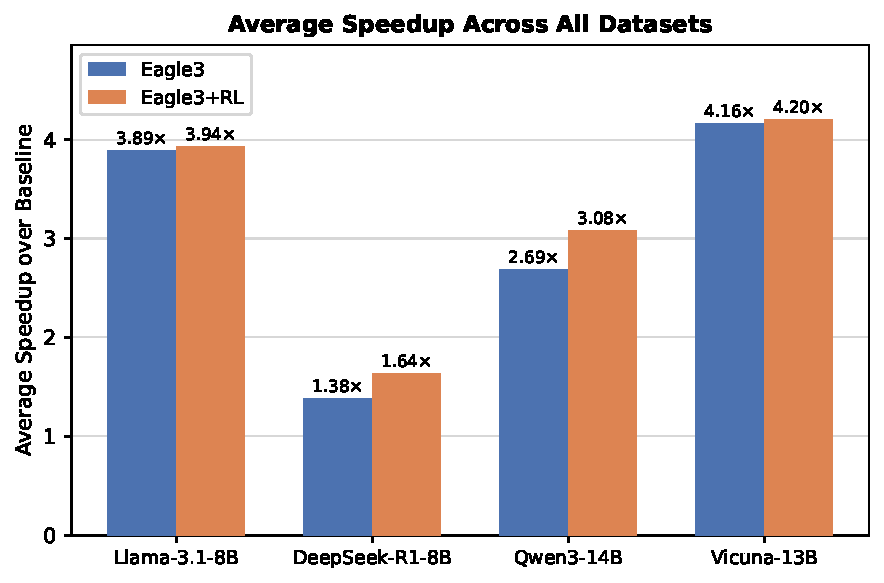
\includegraphics[width=0.76\textwidth]{fig1_avg_speedup.pdf}
  \end{figure}
  \vspace{-0.2cm}
  \begin{block}{Takeaway}
    Eagle3+RL improves all four initial models, with the largest gains on DeepSeek-R1-8B and Qwen3-14B.
  \end{block}
\end{frame}

\begin{frame}
  \frametitle{Qwen3-14B: Strong Cross-Dataset Transfer}
  \begin{columns}[T]
    \column{0.55\textwidth}
    \begin{figure}
      \centering
      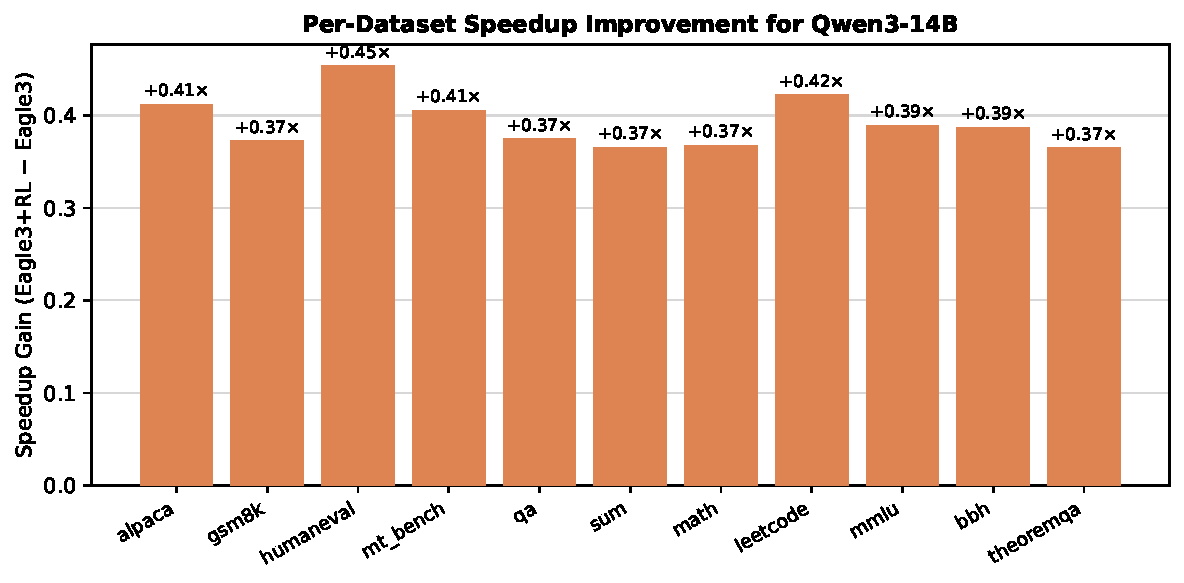
\includegraphics[width=\textwidth]{fig2_qwen_per_dataset.pdf}
    \end{figure}
    \column{0.41\textwidth}
    \begin{block}{Average speedup}
      \begin{itemize}
        \item Eagle3: \speedup{2.69}
        \item Eagle3+RL: \alert{\speedup{3.08}}
        \item Relative gain over Eagle3: 14.5\%
      \end{itemize}
    \end{block}
    \begin{block}{Key point}
      The controller was trained on HumanEval, but every benchmark shows a positive gain.
    \end{block}
  \end{columns}
\end{frame}

\begin{frame}
  \frametitle{Qwen3-32B: Fifth Model Reproduced}
  \begin{table}
    \centering
    \scriptsize
    \setlength{\tabcolsep}{4pt}
    \begin{tabular}{lccc}
      \toprule
      Dataset & Eagle3 & Eagle3+RL & RL/Eagle3 \\
      \midrule
      Alpaca & \speedup{2.99} & \speedup{3.19} & 1.069 \\
      GSM8K & \speedup{3.29} & \speedup{3.45} & 1.047 \\
      HumanEval & \speedup{2.93} & \speedup{3.14} & 1.070 \\
      Math & \speedup{3.36} & \speedup{3.60} & 1.070 \\
      TheoremQA & \speedup{3.15} & \speedup{3.41} & 1.083 \\
      Sum & \speedup{2.49} & \speedup{2.46} & 0.992 \\
      \midrule
      Average, all 11 & \speedup{3.00} & \alert{\speedup{3.16}} & \alert{1.054} \\
      \bottomrule
    \end{tabular}
  \end{table}
  \begin{block}{Takeaway}
    Qwen3-32B under 8-bit quantization benefits from LTD on 10 of 11 datasets, but the average gain is smaller than Qwen3-14B.
  \end{block}
\end{frame}

\begin{frame}
  \frametitle{Throughput Beats Acceptance-Length Maximization}
  \begin{columns}[T]
    \column{0.56\textwidth}
    \begin{figure}
      \centering
      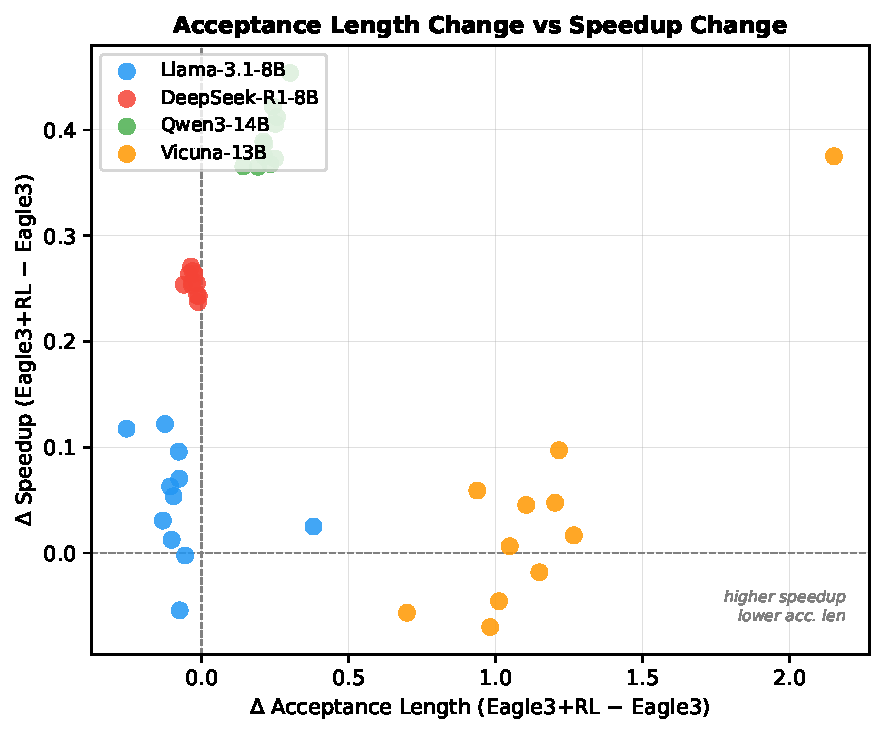
\includegraphics[width=\textwidth]{fig3_acc_vs_speedup.pdf}
    \end{figure}
    \column{0.40\textwidth}
    \begin{block}{Observation}
      Some points improve speedup even when acceptance length decreases.
    \end{block}
    \begin{block}{Interpretation}
      The RL policies are optimizing latency-aware throughput, not simply accepted tokens per speculative step.
    \end{block}
  \end{columns}
\end{frame}

\section{Transfer}

\begin{frame}
  \frametitle{Quantization Transfer Is Mostly Robust}
  \begin{columns}[T]
    \column{0.46\textwidth}
    \begin{table}
      \centering
      \scriptsize
      \setlength{\tabcolsep}{3pt}
      \begin{tabular}{lcccc}
        \toprule
        Policy & bf16 & int4 & int8 & Avg. \\
        \midrule
        bf16 & 1.046 & 1.056 & 1.069 & 1.057 \\
        int4 & \alert{1.118} & 1.060 & 1.057 & \alert{1.078} \\
        int8 & 1.018 & 1.005 & \alert{1.074} & 1.032 \\
        \bottomrule
      \end{tabular}
    \end{table}
    \begin{block}{Summary}
      Average RL/Eagle3 is 1.056 across 36 policy-precision-dataset conditions; only two individual runs regress.
    \end{block}
    \column{0.50\textwidth}
    \begin{figure}
      \centering
      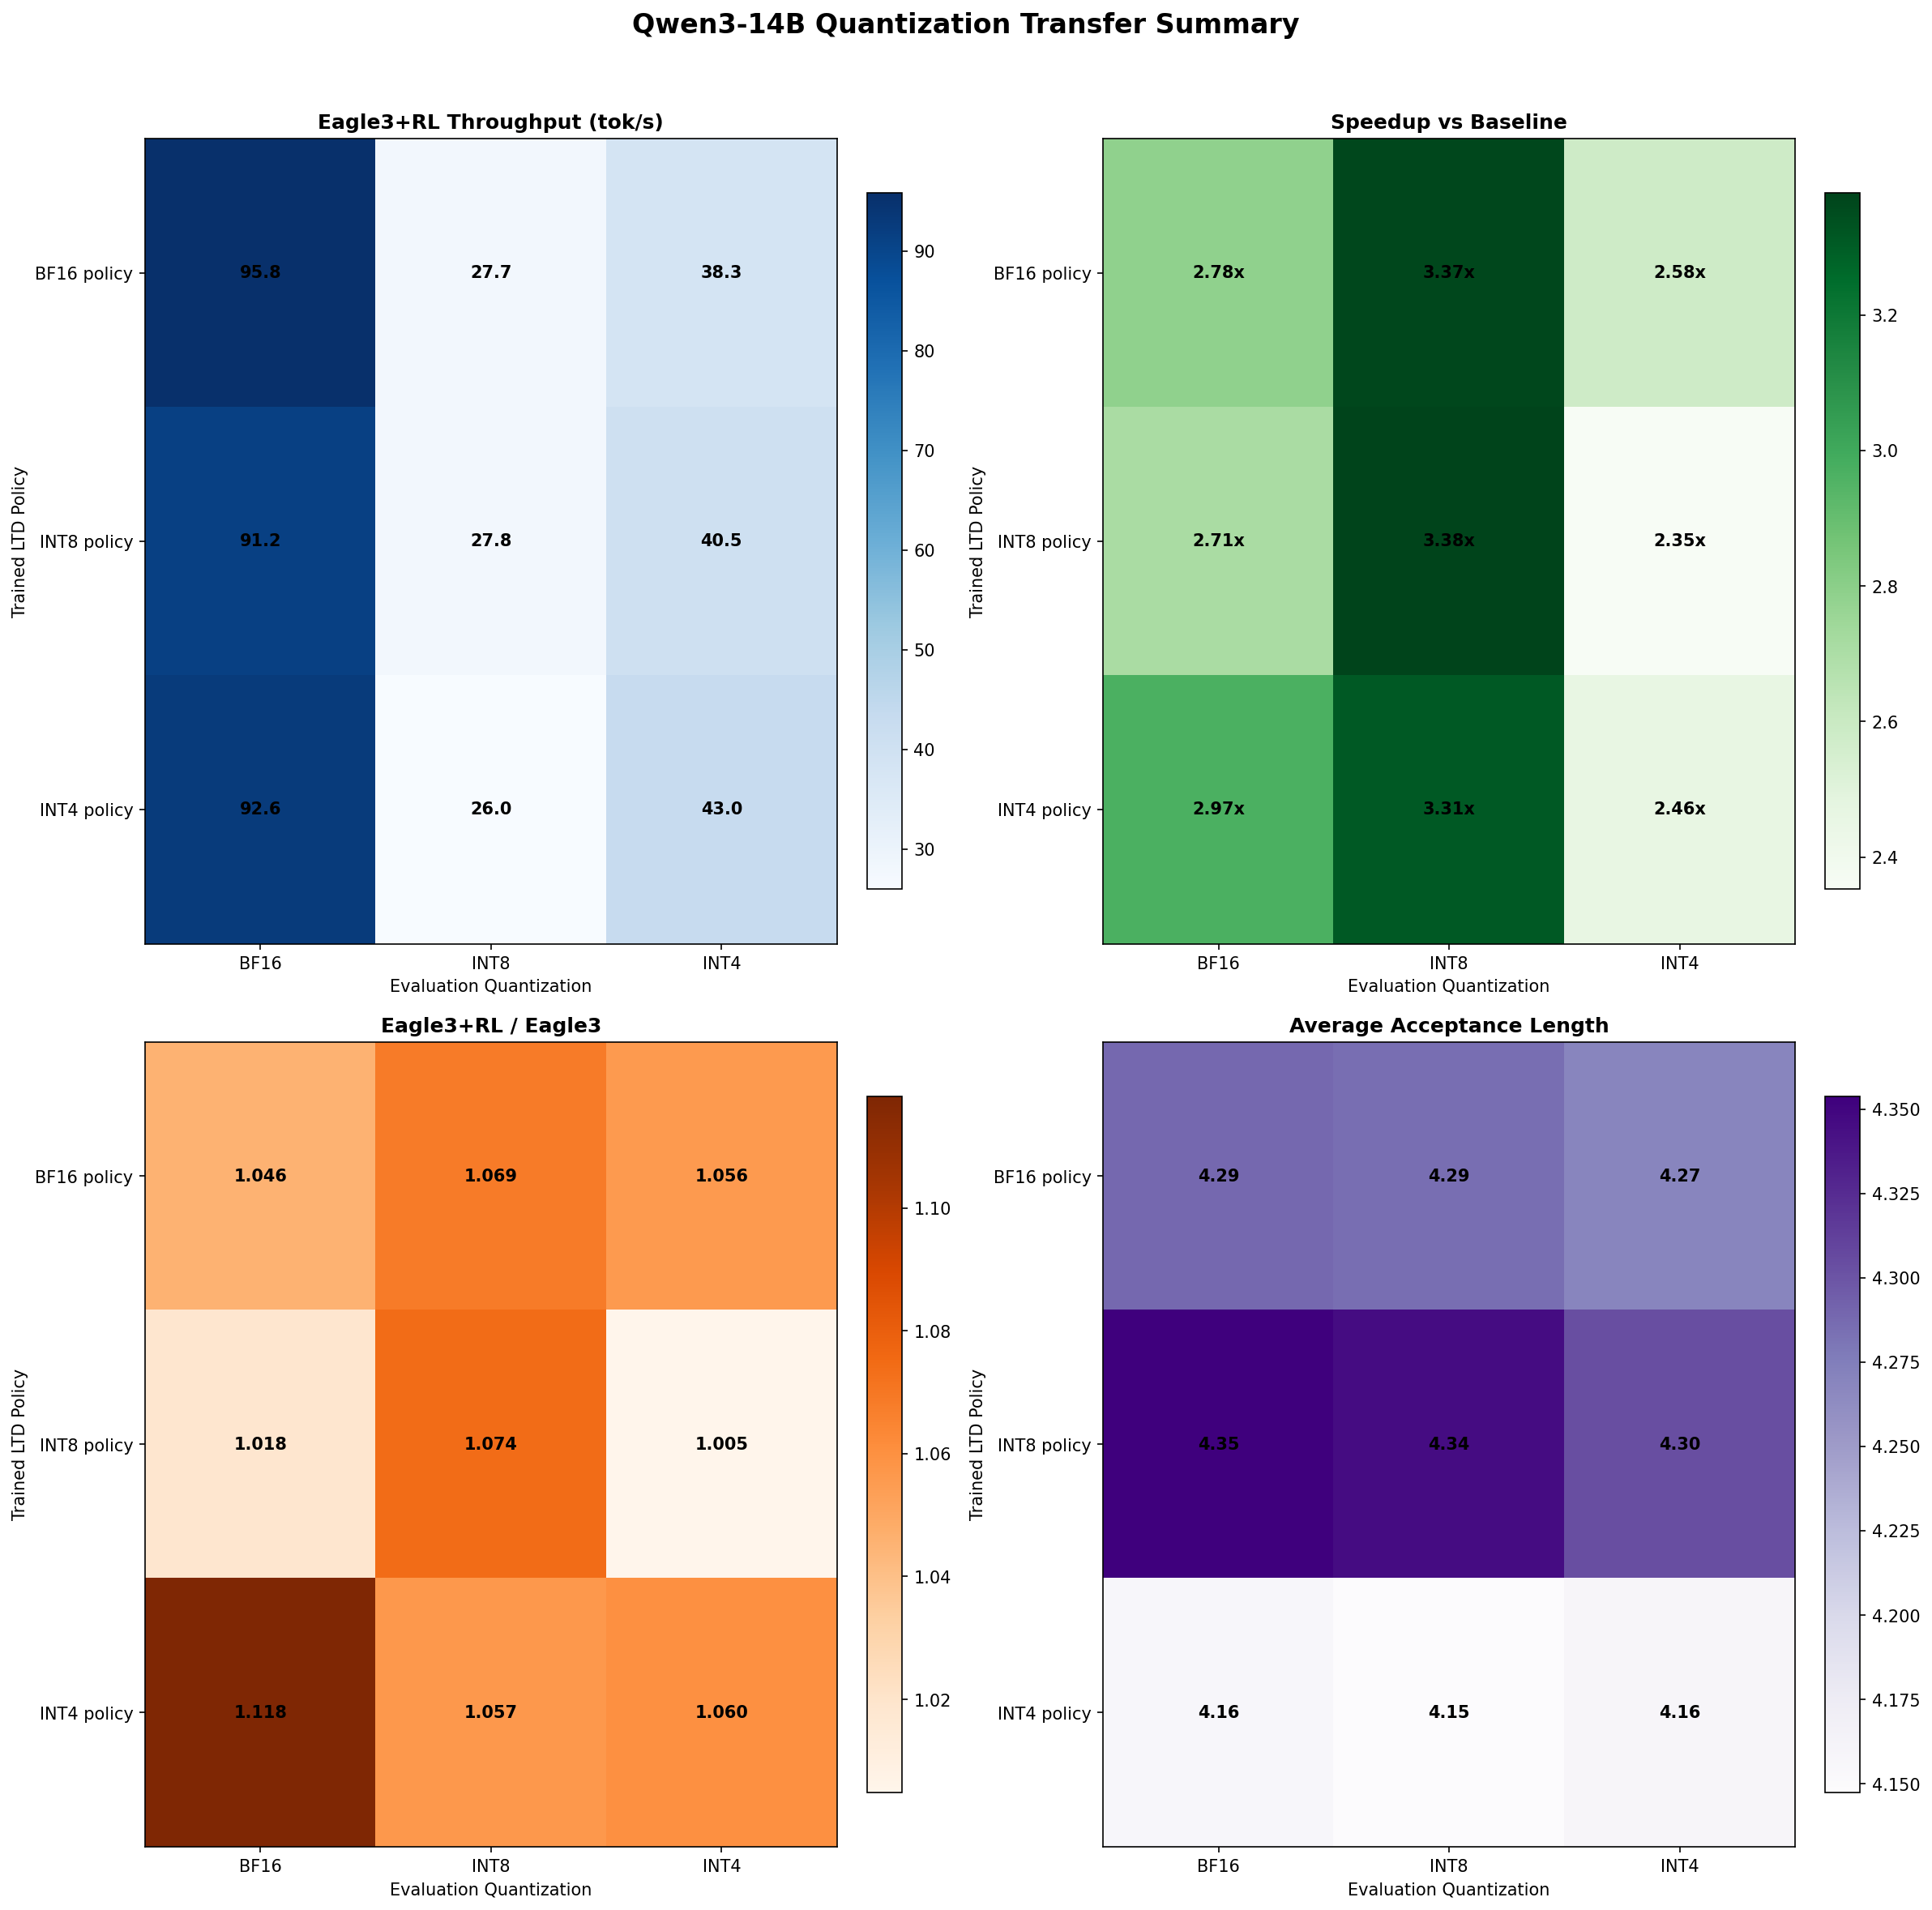
\includegraphics[width=\textwidth]{quant_transfer_summary_charts.png}
    \end{figure}
  \end{columns}
\end{frame}

\begin{frame}
  \frametitle{Hardware Transfer Is Brittle}
  \begin{columns}[T]
    \column{0.45\textwidth}
    \begin{table}
      \centering
      \scriptsize
      \setlength{\tabcolsep}{3pt}
      \begin{tabular}{lccc}
        \toprule
        Train GPU & Eagle3 & RL & RL/E3 \\
        \midrule
        A5090 & \speedup{2.55} & \speedup{1.76} & 0.693 \\
        H100 & \speedup{2.55} & \speedup{1.89} & 0.739 \\
        \bottomrule
      \end{tabular}
    \end{table}
    \begin{alertblock}{Takeaway}
      Policies trained on H100 or A5090 are still faster than autoregressive decoding, but fail to beat static Eagle3 on RTX A6000.
    \end{alertblock}
    \column{0.51\textwidth}
    \begin{figure}
      \centering
      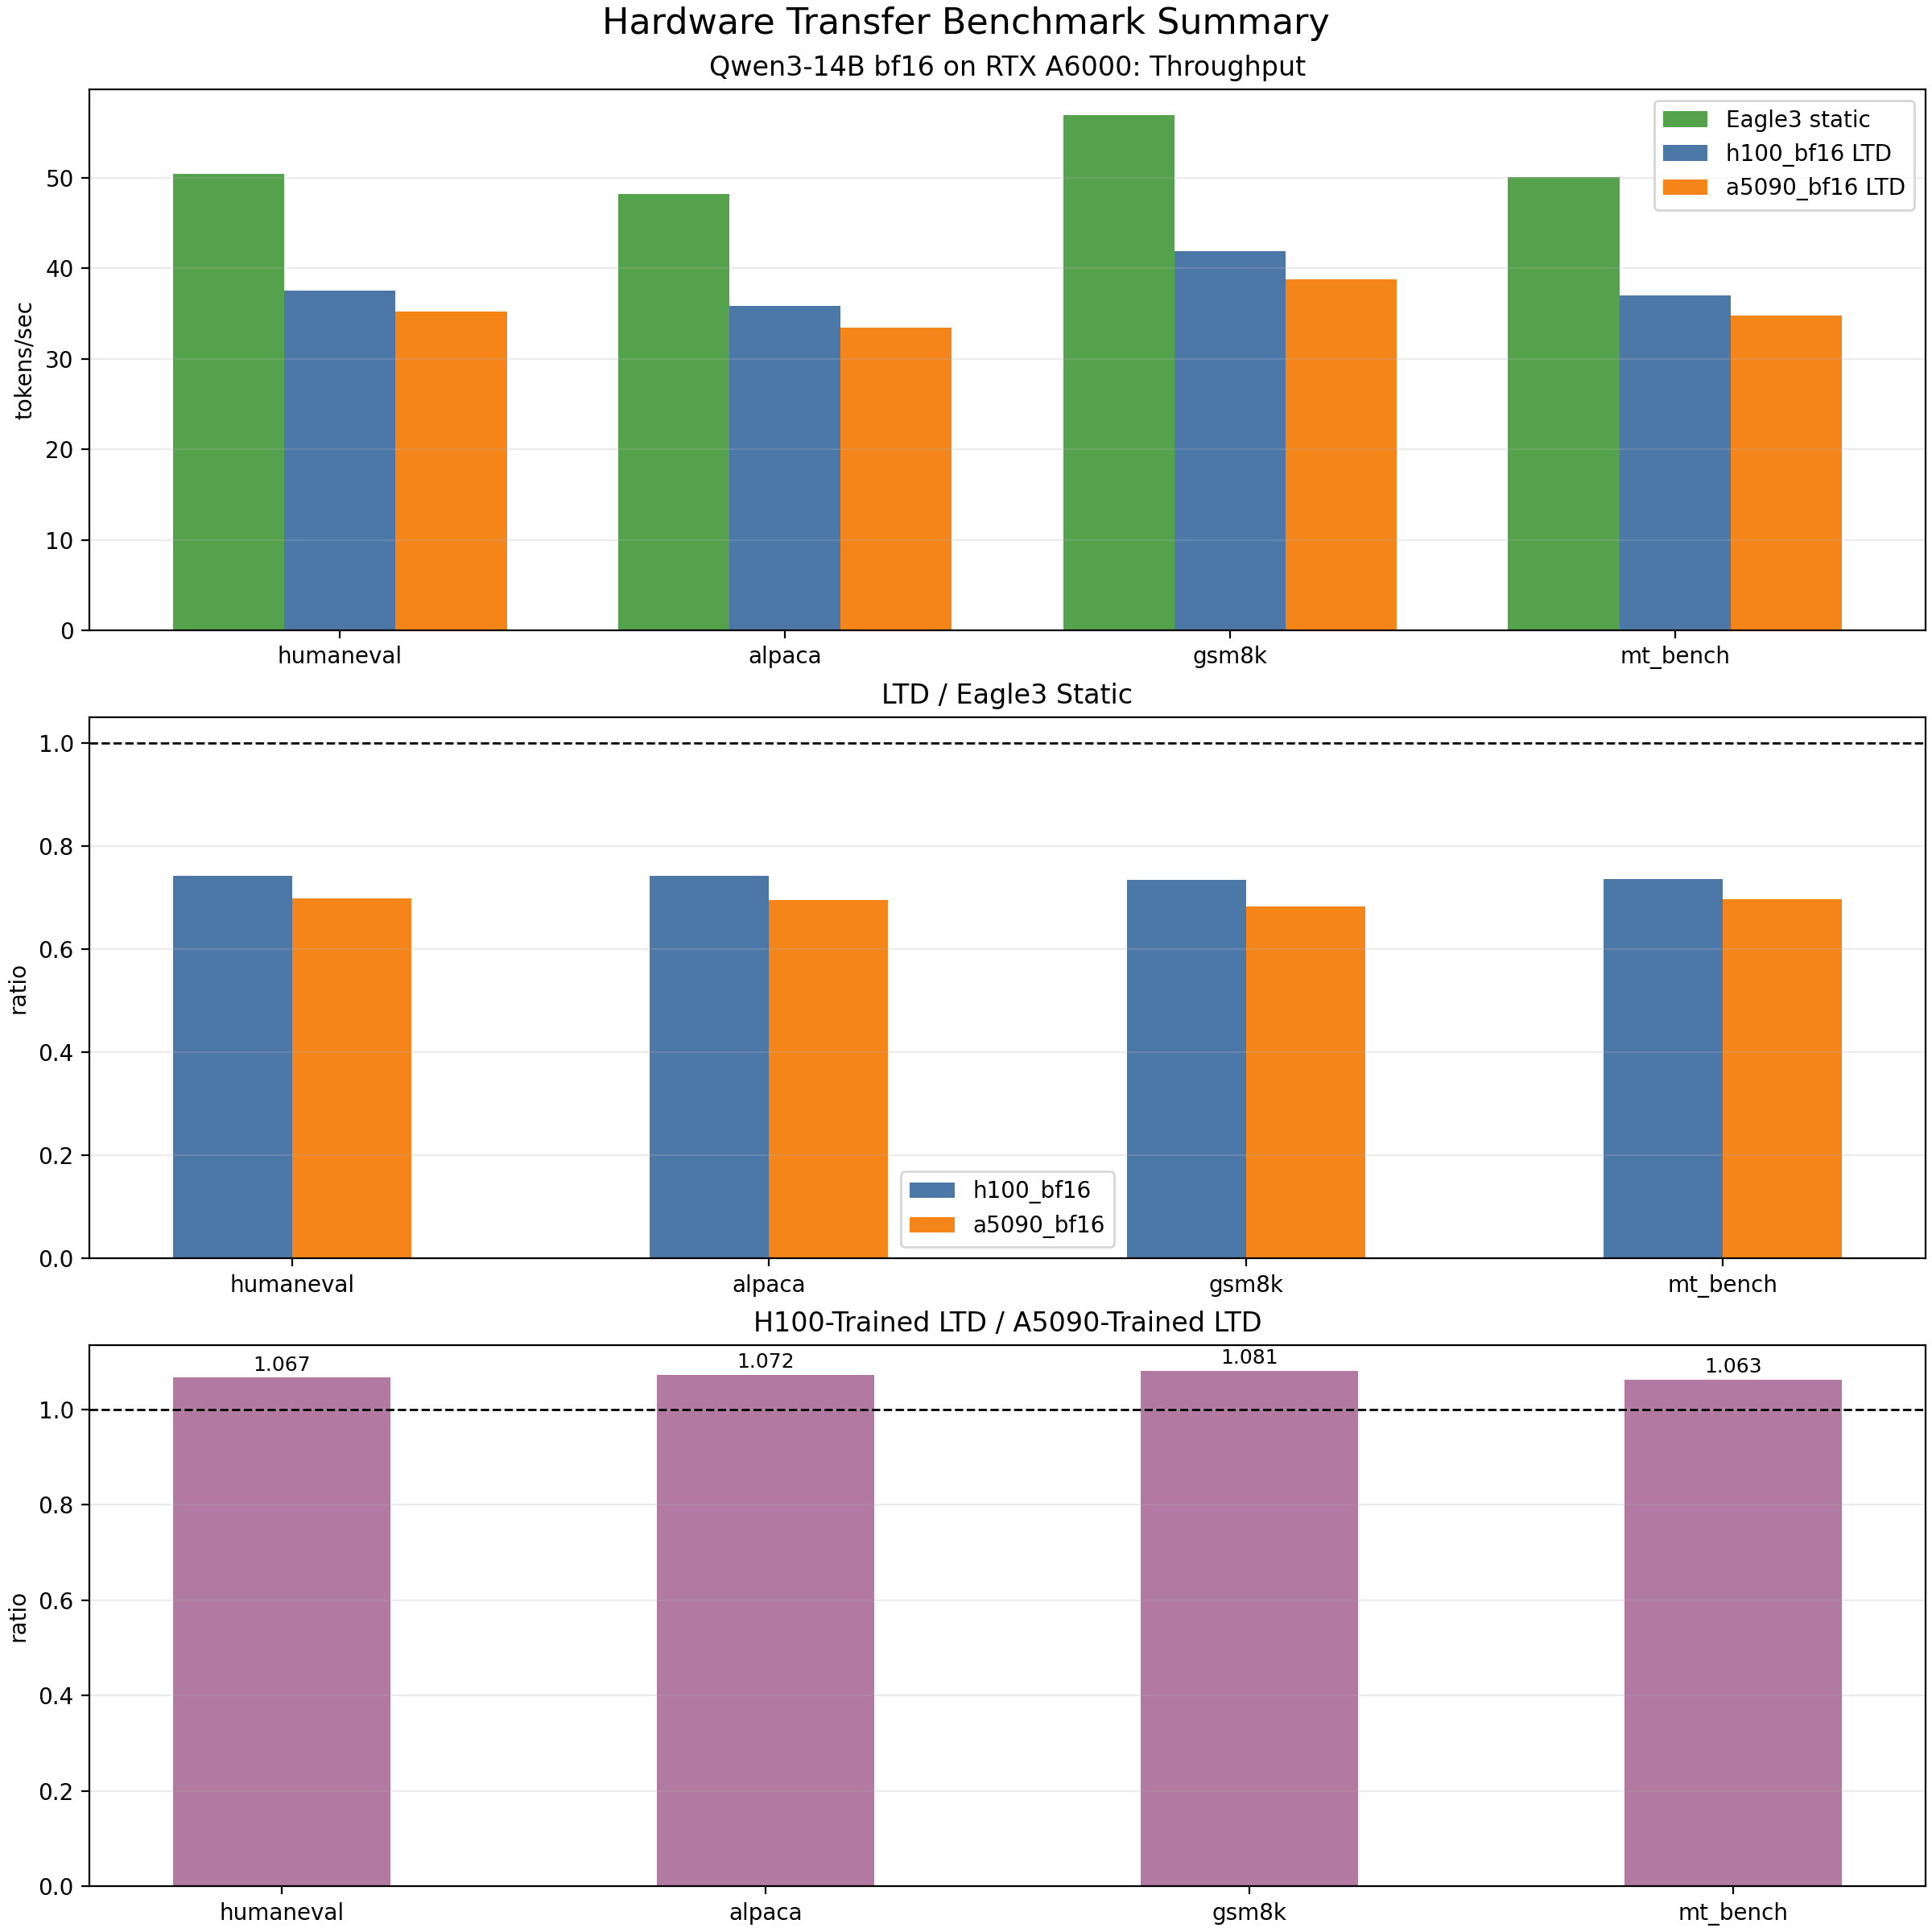
\includegraphics[width=\textwidth]{hardware_transfer_summary_charts.png}
    \end{figure}
  \end{columns}
\end{frame}

\begin{frame}
  \frametitle{Why Hardware Transfer Fails}
  \begin{itemize}
    \item The reward learns a hardware-specific latency surface.
    \item Larger verification batches are amortized differently across GPUs.
    \item Memory bandwidth and kernel overhead shift the best size-depth trade-off.
    \item A policy that is optimal on the training GPU can choose actions that are too costly on the target GPU.
  \end{itemize}

  \vspace{0.3cm}
  \begin{block}{Implication}
    Quantization transfer looks feasible, but hardware transfer likely needs hardware-conditioned observations or lightweight target-GPU fine-tuning.
  \end{block}
\end{frame}

\section{Deployment}

\begin{frame}
  \frametitle{Naive Two-GPU Model Parallelism}
  \begin{table}
    \centering
    \small
    \setlength{\tabcolsep}{5pt}
    \begin{tabular}{lccccc}
      \toprule
      Setting & Base tp & E3 tp & RL tp & RL speedup & RL/E3 \\
      \midrule
      1 GPU & 5.60 & 16.75 & 17.67 & \speedup{3.16} & 1.054 \\
      2 GPUs & 5.11 & 15.36 & 16.19 & \speedup{3.17} & 1.053 \\
      \bottomrule
    \end{tabular}
  \end{table}

  \begin{block}{Takeaway}
    The relative LTD gain is preserved under layer sharding, but absolute throughput drops by about 8\%. Naive model parallelism helps placement more than latency.
  \end{block}
\end{frame}

\begin{frame}
  \frametitle{Saturation Explains Small Gains}
  \begin{columns}[T]
    \column{0.55\textwidth}
    \begin{figure}
      \centering
      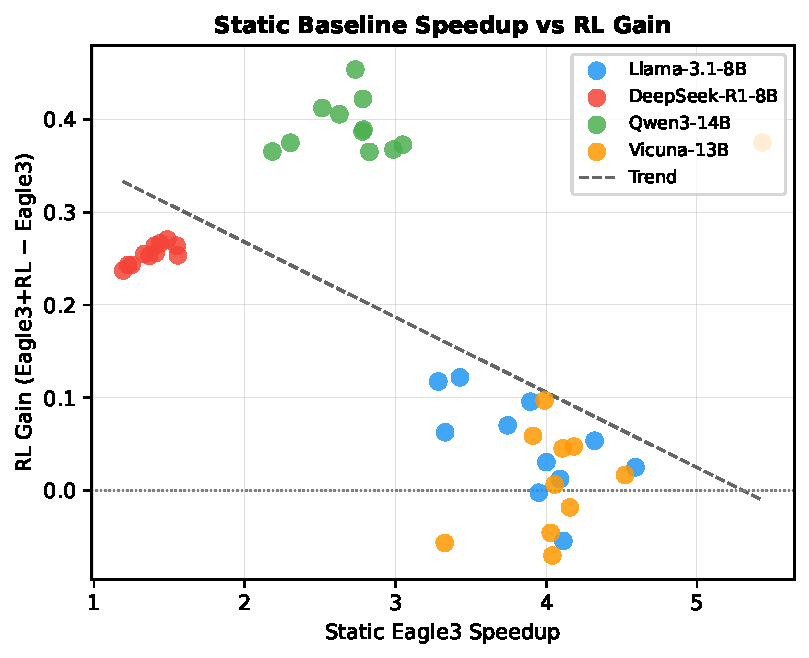
\includegraphics[width=\textwidth]{fig4_saturation.pdf}
    \end{figure}
    \column{0.41\textwidth}
    \begin{block}{Pattern}
      Stronger static Eagle3 baselines leave less room for RL improvement.
    \end{block}
    \begin{block}{Examples}
      \begin{itemize}
        \item Vicuna and Llama: static baseline already strong.
        \item DeepSeek and Qwen3-14B: larger adaptive-control gains.
        \item Qwen3-32B: positive but modest under 8-bit.
      \end{itemize}
    \end{block}
  \end{columns}
\end{frame}

\section{Conclusion}

\begin{frame}
  \frametitle{Main Takeaways}
  \begin{enumerate}
    \item We reproduced LTD on five target models, including Qwen3-32B under 8-bit quantization.
    \item LTD improves same-hardware, same-precision EAGLE-3 throughput in most settings.
    \item Quantization transfer is mostly robust across bf16, int4, and int8.
    \item Hardware transfer is brittle: throughput-optimized policies encode GPU-specific trade-offs.
    \item Naive two-GPU sharding preserves relative LTD gains but does not improve absolute throughput.
  \end{enumerate}
\end{frame}

\begin{frame}
  \frametitle{Next Steps}
  \begin{itemize}
    \item Evaluate temperature sampling, not only greedy decoding.
    \item Analyze policy action distributions across tasks and deployment conditions.
    \item Add hardware-conditioned features or lightweight fine-tuning for target GPUs.
    \item Explore true distributed speculative decoding with pipeline or tensor parallelism.
  \end{itemize}

  \vfill
  \centering
  \Large Questions?
\end{frame}

\end{document}
